\section{How wrong is the reported number?}
\label{sec:inflation}

\paragraph{Data.}
\emph{CIFAR-Aug} is a controlled pre-augmented release: $2{,}000$ CIFAR-10 training photographs~\citep{krizhevsky2009cifar}, each with $15$ edited copies at three strengths (weak: colour and flips; medium: plus rotations and crops; strong: plus one or two filters; Appendix~\ref{app:data}). Because the sources are known, we can also score every model on $3{,}000$ \emph{fresh} CIFAR-10 test photographs: the accuracy a deployment would see. \emph{Leaf-A} ($600$ sources $\times$ $15$ variants) and \emph{Leaf-B} ($850\times16$) are real public releases of field-crop leaf photographs, three classes each, whose file names encode the source; their variants include geometric edits and heavy filters (Figure~\ref{fig:concept}a). In \emph{COVID-CXR}~\citep{cohen2020covid} groups are patients; we use $699$ frontal radiographs of $424$ patients (COVID-19 vs.\ other findings).

\paragraph{Models.}
We use frozen ImageNet backbones (MobileNetV3-Large~\citep{howard2019mobilenetv3} in the main text, EfficientNet-B0~\citep{tan2019efficientnet} in Appendix~\ref{app:backbones}) with two heads that bracket how strongly a model can exploit a sibling: a 1-nearest-neighbour classifier (pure memory) and an $\ell_2$-regularised linear probe. Appendix~\ref{app:finetune} adds full fine-tuning. Every number is a mean over at least three seeds; the seed controls the split.

\begin{figure}[t]
  \centering
  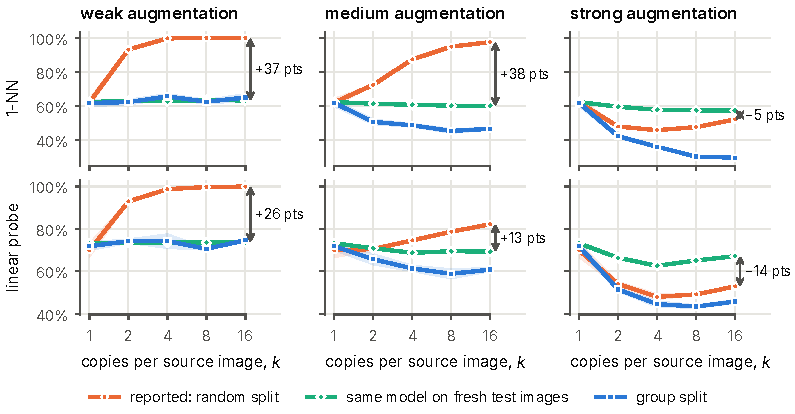
\includegraphics[width=\linewidth]{figs/fig_inflation.pdf}
  \caption{\textbf{Reported accuracy can be far above or below the truth.} CIFAR-Aug, $2{,}000$ sources, frozen MobileNetV3. Orange: the number a paper would report (random split). Green: the same model scored on fresh CIFAR-10 test photographs. Blue: a group split, which removes the leak but still tests on edited copies. Bands: 95\% intervals over seeds (often thinner than the line).}
  \label{fig:inflation}
\end{figure}

\paragraph{The error has two sources and either sign.}
Measured exposure matches \Eqref{eq:exposure} (Appendix Table~\ref{tab:exposure}): $100\%$ on both leaf releases and on CIFAR-Aug for $k\ge8$, \numCovidQ{} on COVID-CXR. Figure~\ref{fig:inflation} separates the two errors. With weak edits the reported 1-NN accuracy reaches \numWeakKnnRep{} while the same model scores \numWeakKnnFresh{} on fresh photographs; the linear probe is inflated from \numWeakLpFresh{} to \numWeakLpRep{}. Exposure saturates by $k=4$ (Proposition~\ref{prop:exposure}), yet the reported accuracy keeps rising with $k$ as more copies of each test image enter training, and the gap is larger for smaller releases: with medium edits the linear-probe gap is \numSizeGapSmall{} points for $500$ sources and \numSizeGapLarge{} for $2{,}000$ (Appendix Table~\ref{tab:datasize}). With strong edits the sign flips: the test set is now dominated by filtered images that are harder than real photographs, and the reported linear-probe accuracy (\numStrongLpRep{}) is \emph{below} the fresh accuracy (\numStrongLpFresh{}). A group split (blue) removes the leak but inherits this second bias; scoring the group split on the unedited member of each test group recovers the fresh accuracy (Appendix~\ref{app:orig}). The reported number is therefore not even a bound: it is a mixture of an optimistic and a pessimistic error whose balance depends on how the release was made.

\paragraph{Real releases.}
On the real data (Appendix Table~\ref{tab:real}), random splits overstate group-split accuracy by \numLeafALpGap{} (Leaf-A) and \numLeafBLpGap{} (Leaf-B) points for the linear probe and by up to \numLeafBKnnGap{} points for 1-NN; patient leakage in COVID-CXR adds \numCovidLpGap{} points. End-to-end fine-tuning, which can memorise individual images~\citep{zhang2017rethinking,feldman2020memorization}, does not remove them (Appendix~\ref{app:finetune}): on CIFAR-Aug (medium, $k=8$) a fine-tuned MobileNetV3 reports \numFtCMedRandom{} under a random split but reaches \numFtCMedRandomFresh{} on fresh photographs (EfficientNet-B0: \numFtCMedEffRandom{} vs.\ \numFtCMedEffRandomFresh{}; 3 seeds), and on Leaf-B the random split reports \numFtLeafBRandom{} where the group split gives \numFtLeafBGroup{}, understating the error rate about \numFtLeafBErrRatio{}-fold.


\paragraph{Which siblings are exploited?}
Figure~\ref{fig:exploit} bins test images of a random split by the cosine similarity, in the model's own embedding, between each image and its closest training sibling. When that sibling is dissimilar, accuracy is close to, or on the leaf releases even below, the group-split accuracy: these are mostly heavily filtered copies, not helped by their siblings. As the sibling gets closer, accuracy climbs steeply towards $100\%$. A detector therefore need not find every sibling, only the ones the model can use.

\begin{figure}[t]
  \centering
  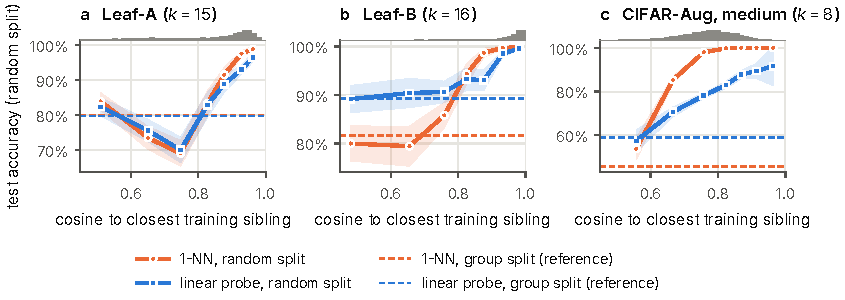
\includegraphics[width=\linewidth]{figs/fig_exploit.pdf}
  \caption{\textbf{Inflation comes from close siblings.} Accuracy of test images in a random split, binned by the cosine between each image and its closest training sibling in the probe's embedding (bins with $\ge30$ images; bands are 95\% binomial intervals; grey bars show how test images are distributed over the bins). Dashed lines: accuracy under a group split.}
  \label{fig:exploit}
\end{figure}
